%%%%%%%%%%%%%%%%%%%%%%%%%%%%%%%%%%%%%%%%%
% Thin Sectioned Essay
% LaTeX Template
% Version 1.0 (3/8/13)
%
% This template has been downloaded from:
% http://www.LaTeXTemplates.com
%
% Original Author:
% Nicolas Diaz (nsdiaz@uc.cl) with extensive modifications by:
% Vel (vel@latextemplates.com)
%
% License:
% CC BY-NC-SA 3.0 (http://creativecommons.org/licenses/by-nc-sa/3.0/)
%
%%%%%%%%%%%%%%%%%%%%%%%%%%%%%%%%%%%%%%%%%

%----------------------------------------------------------------------------------------
%	PACKAGES AND OTHER DOCUMENT CONFIGURATIONS
%----------------------------------------------------------------------------------------

\documentclass[a4paper, 21pt]{article} % Font size (can be 10pt, 11pt or 12pt) and paper size (remove a4paper for US letter paper)

\usepackage[protrusion=true,expansion=true]{microtype} % Better typography
\usepackage{graphicx} % Required for including pictures
\usepackage{wrapfig} % Allows in-line images
\usepackage[utf8]{inputenc}  % UTF8 characters
\DeclareGraphicsExtensions{.pdf,.png,.jpg}
\graphicspath{{logos/}{figs/}}
\usepackage{caption}
\usepackage{mathpazo} % Use the Palatino font
\usepackage[T1]{fontenc} % Required for accented characters
\usepackage{url} % For URLs
\usepackage{listings}        % code listings
\usepackage{color} 
\usepackage{float}  
\linespread{1.05} % Change line spacing here, Palatino benefits from a slight increase by default

\makeatletter
% \renewcommand\@biblabel[1]{\textbf{#1.}} % Change the square brackets for each bibliography item from '[1]' to '1.'
\renewcommand{\@listI}{\itemsep=0pt} % Reduce the space between items in the itemize and enumerate environments and the bibliography

\renewcommand{\maketitle}{ % Customize the title - do not edit title and author name here, see the TITLE block below
\begin{flushright} % Right align
{\LARGE\@title} % Increase the font size of the title

\vspace{50pt} % Some vertical space between the title and author name

{\large\@author} % Author name
\\\@date % Date

\vspace{40pt} % Some vertical space between the author block and abstract
\end{flushright}
}

%----------------------------------------------------------------------------------------
%	TITLE
%----------------------------------------------------------------------------------------

\title{\textbf{Handbook for Matlab GUI}\\ % Title
Ranging between two devices} % Subtitle

\author{\textsc{Pablo del Hoyo Rodríguez} % Author
\\{\textit{Technische Universität Hamburg-Harburg}}} % Institution

\date{\today} % Date

%----------------------------------------------------------------------------------------

\begin{document}

\maketitle % Print the title section

%----------------------------------------------------------------------------------------
%	ABSTRACT AND KEYWORDS
%----------------------------------------------------------------------------------------

%\renewcommand{\abstractname}{Summary} % Uncomment to change the name of the abstract to something else

\begin{abstract}
This document presents the detailed information about the program used to range between two Pozyx devices. The program consists of a Graphical User Interface (GUI) for Matlab which easily ranges and set a real distance between two Pozyx devices. The GUI provides the functionalities to restrict the time or the number of samples. Also, it plots the error distribution and its main data.
\end{abstract}

\hspace*{3,6mm}\textit{Keywords:} Matlab, GUI, Arduino, Pozyx, Ranging % Keywords

\vspace{30pt} % Some vertical space between the abstract and first section

\tableofcontents
\newpage
%----------------------------------------------------------------------------------------
%	ESSAY BODY
%----------------------------------------------------------------------------------------

\section{Prerequisites}


As the program will provide a communication between the Arduino board and the computer, two parts will be considered in order to make the installation the Matlab side and the Arduino side:\\
\begin{figure}[!hbbp]
\begin{center}

\includegraphics[scale=0.8]{fig/matlab_arduino.png}
\end{center}
\caption{Both sides of the program}
\end{figure}

For the Matlab site it is required:
\begin{itemize}
\item Matlab R2016a (older versions may be valid)
\item Arduino Support from Matlab: package to communicate with an Arduino. The installation steps are available at reference \cite{Matlab:Arduino} and is usually installed by double clicking the package download file.
\end{itemize}

For the Arduino side is required:
\begin{itemize}
\item Arduino Uno x1
\item USB-B Cable x1
\item Pozyx Shield for Arduino
\item  The Arduino IDE and Pozyx Arduino Library: the installation steps are provided at reference \cite{Arduino:Started}
\item Pozyx Anchor x1 (or another Pozyx Shield)
\item  USB-C Cable x1 (or another USB-B Cable and Arduino UNO)
\end{itemize}

%------------------------------------------------

\section{Script Files}
The ranging.zip file is provided with the following files:
\begin{table}[]
\centering
\begin{tabular}{|l|l|}
\hline
\textbf{File}                 & \textbf{Description}                                                                                                                      \\ \hline
HandbookRange.pdf             & This file, description and a tutorial of the program                                                                                      \\ \hline
\textbf{read.m}               & Main Matlab file. To be executed                                                                                                          \\ \hline
read.fig                      & Matlab Figure for the GUI                                                                                                                 \\ \hline
ready\_to\_range\_arduino.ino & \begin{tabular}[c]{@{}l@{}}Scketch to run onto the Arduino, do the ranging\\ See section \ref{se:arduino} for more details\end{tabular} \\ \hline
(subfolder) functions         & Some Matlab functions including these below                                                                                               \\ \hline
changeVisibility.m            & Hide buttons to prevent some errors                                                                                 \\ \hline
checkIfFinished.m               & Handles a flag to stop the ranging function                                                                                               \\ \hline
initArduino.m                 & Initialize serial communication Matlab-Arduino                                                                                  \\ \hline
updatePorts.m                  & Update the communication ports available (USB)                                                                                            \\ \hline
\end{tabular}
\caption{List of files.}
\end{table}
\newpage
%------------------------------------------------


\section{Arduino Setup}\label{se:arduino}
Before running the main Matlab file (\textit{read.m}), some restrictions about the scenario have to be taken into consideration:
\begin{itemize}
\item First and most important, the identifier of the destination device must be specified in the sketch \textit{ready\_to\_range\_arduino.ino} as well as the UWB channel (1,2,3,4,5 or 7). This can be done by editing the following lines:
\begin{lstlisting}[language=c, breaklines=true, commentstyle=\color{blue}, basicstyle=\ttfamily\small]
// Edit with your scenario:
uint16_t destination_id = 0x6670;     
int uwb_channel = 1;
\end{lstlisting}
\item There is a minimum separation distance that allows the ranging. Apparently, distances lower than 20 mm provides always a zero estimator.
\item As there is some processing time in order to present all the information, \textbf{there is a delay between the current data being read and that one being represented}. So the ranging results are not strictly represented in real time. However, all the data is considered when the execution of the code is finished.
\end{itemize}

%------------------------------------------------
\section{Overview}
Once all the previous sections have been explained, the procedure to run the interface is described. The file localize.m has to be opened (by double-clicking or with the Matlab interface). After setting the path to the one corresponding to this project, the file can be executed (F5). This will open the interface, whose appearance is shown in the screenshot below:\\

\begin{figure}[H]
\begin{center}
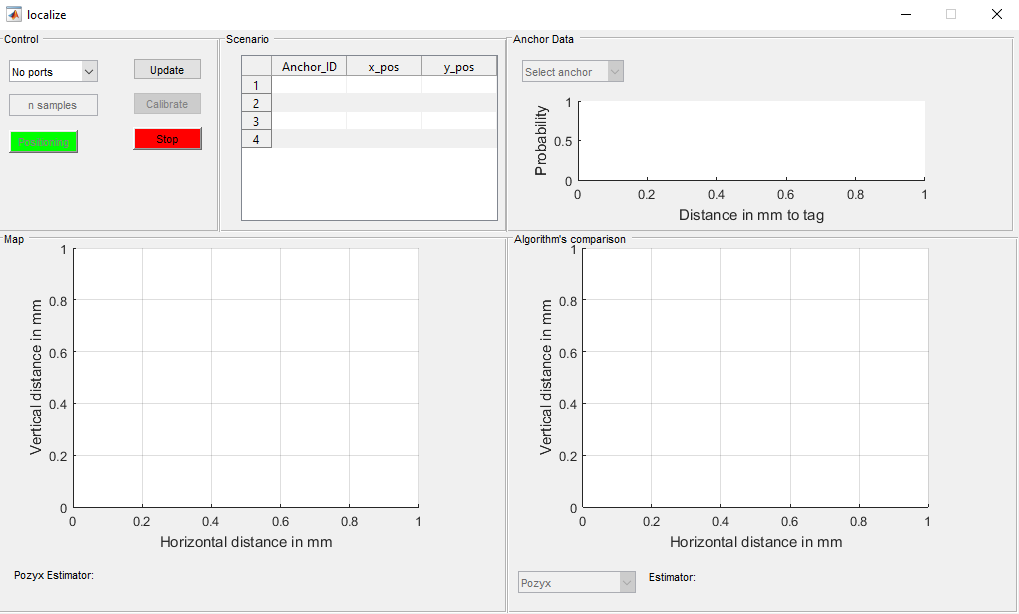
\includegraphics[scale=.7]{fig/ss_ov.png}
\end{center}
\caption{The interface of the program running on Windows 10.}
\end{figure}

The next sections will indicate the functionalities of the program in detail

\section{Control}
This section explain all the possibilities for the problem setup:
\begin{figure}[!hbbp]
\begin{center}
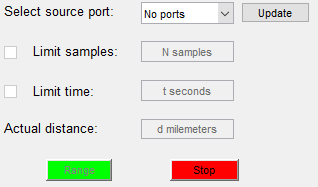
\includegraphics[scale=.9]{fig/ss_control.png}
\end{center}
\caption{The control panel.}
\end{figure}

\begin{itemize}
\item The list of ports pop-up: indicates the currently connected COM ports. In case that nothing is connected, the execution of the code is not permitted. \textbf{Please make sure that the selected COM port is the one corresponding to the SOURCE Arduino running the \textit{ready\_to\_range\_arduino.ino sketch}}.
\item The update button: as its name indicates, updates the available ports and enable the buttons if at least one is connected:
\begin{figure}[H]
\begin{center}
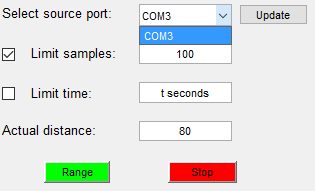
\includegraphics[scale=.8]{fig/ss_control2.png}
\end{center}
\caption{Setting the port after updating the list.}
\end{figure}
\item n samples text box: if it is checked, this sets the number of samples that will be used for the ranging. \textbf{Please make sure that only positive integers are considered}. Other values may arise unconsidered errors. Also notice that larger values produces longer calculation times and larger delays between the current ranging and the one being represented.
\item t time text box: if it is checked, this sets the number of samples that will be used for the ranging. \textbf{Please make sure that only positive numbers are considered}. Other values may arise unconsidered errors. Also notice that larger values produces longer calculation times and larger delays between the current ranging and the one being represented.
\item actual distance text box: this will set the real distance between the devices. See section \ref{se:results} for more details. This is the parameter $d(t)$.
\item the range button: it sends to the tag a command to range to de destination device, shwoing the information as soon as it is processed. If is limited by the number of samples or by the time (or both), the current progress will be displayed. If not, it is required to press the stop button. Once the ranging finishes, a matrix containing n samples with the number of sample, the time in ms and the distance in mm is printed.
\item the stop button: interrupts the execution of the code, for example in the case a very large number of samples was set and the process is wanted to be closed.
\end{itemize}

%------------------------------------------------

\section{Results}\label{se:results}
The left plot shows the evolution of the distance over time, defined as $\hat{d}(t)$. Thus, the green graph represents the distance between the tag a the destination calculated by the Pozyx:
\begin{figure}[H]
\begin{center}
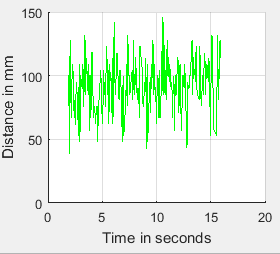
\includegraphics[scale=.8]{fig/d.png}
\end{center}
\caption{Distance $d(t)$ over time.}
\end{figure}

The right plot represents the histogram of the error distance defined as $e(t) = \hat{d}(t)-d(t)$. So the blue bars represent the number of appearances for each error:
\begin{figure}[H]
\begin{center}
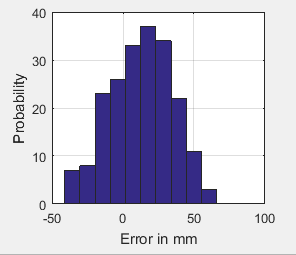
\includegraphics[scale=.9]{fig/e.png}
\end{center}
\caption{Error $e(t)$ over time. Seems to be Gaussian.}
\end{figure}

Finally the rigth data displays the most relevant information of the error distribution, including the mean and the variance:
\begin{figure}[H]
\begin{center}
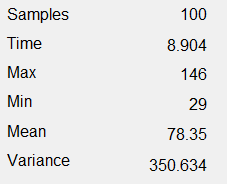
\includegraphics[scale=.9]{fig/e2.png}
\end{center}
\caption{Data of error $e(t)$ over time. Seems to be Gaussian.}
\end{figure}

\section{Future Work}
Once the program has been presented, it has been observed that many functionalities can be implemented with the interface.\\

It would be interesting to provide a tool to manually set the destination device id. However, it was difficult to do it as the transmitted data is hexadecimal throughout a serial bus, interpreting the Arduino sketch the wrong id.\\

Also, some synchronization issues have been observed, as the data is read faster in some computers. If there is no data to be read, the code waits a time until it is again available, defining a buffer. However, it has been observed some unsuitability with these waiting times. Improve this buffer to work correctly in every scenario and computer is an important issue to be solved.\\

%----------------------------------------------------------------------------------------
%	BIBLIOGRAPHY
%----------------------------------------------------------------------------------------

\bibliographystyle{unsrt}

\bibliography{sample}

%----------------------------------------------------------------------------------------

\end{document}